\section{习题}\label{sec:习题08}
\begin{enumerate}
    \item \circleone 光学中费马原理的一个推论是光从
          折射率为$\eta_1$的介质中一点$\bm{p}_1$传播到
          折射率为$\eta_2$的介质中另一点$\bm{p}_2$时遵循的路径
          会最小化从第一个点到第二个点的耗时。斯涅尔定律可以直接从
          这个事实推导出来。考虑光在被一平面边界分开的
          两点$\bm{p}_1$和$\bm{p}_2$之间传播。
          光从$\bm{p}_1$传播到$\bm{p}_2$时可能通过边界上的任意一点
          (见\reffig{8.25}展示的\sidenote{译者注:原文图注把点$\bm{p}'$误写为点$\bm{p}$,已修正。}
          两个可能的点$\bm{p}'$与$\bm{p}''$)。
          回想光在具有恒定折射率的介质中于两点间传播的耗时正比于
          它们间的距离乘以介质折射率。利用该事实,证明
          \sidenote{译者注:可参见笔者补充的证明\ref{prove:FermatSnell}。}
          边界上能最小化从$\bm{p}_1$到$\bm{p}_2$的传播时间的
          点$\bm{p}'$满足$\eta_1\sin\theta_1=\eta_2\sin\theta_2$.
          \begin{figure}[htbp]
              \centering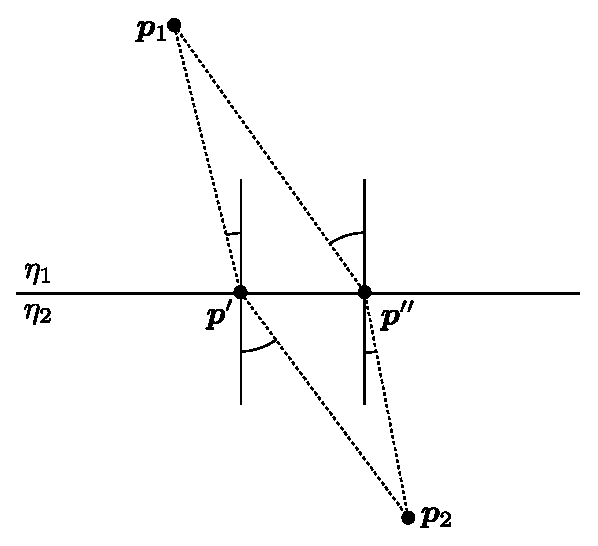
\includegraphics[width=0.5\linewidth]{Pictures/chap08/Fermatsprinciple.eps}
              \caption{斯涅尔定律的推导。斯涅尔定律可以用费马原理推导出,
                  即光在两点间传播时会遵循时间最短的路径。
                  因而两种介质边界上的折射角$\theta$可被证明最小化了
                  从点$\bm{p}_1$到点$\bm{p}'$的耗时加上从该点到点$\bm{p}_2$的耗时。}
              \label{fig:8.25}
          \end{figure}
    \item \circlethree 阅读论文\citet{10.1109/38.62695}与\citet{10.1145/192161.192204},
          并运用其描述的一些技术修改pbrt以对光的偏振效应建模。
          构建场景并渲染它们的图像以说明当精确建模偏振时产生的显著差异。
    \item \circlethree 用含有大量镜像微面的粗糙平面构造一个含有真实几何模型的场景
          \footnote{必须用面光源而不是点光源或定向光源,因为镜像曲面中看到的这些光源有细微差异。
              对于pbrt所用的光传输算法,镜像曲面中的无穷小点光源是永远不可见的。
              这是光线追踪渲染器的典型局限性且实践中通常不会带来麻烦。}。
          把相机置于场景中使得每个像素区域内都有非常大量的微面,
          用成百上千的像素样本来渲染该场景图像。比较使用平坦曲面与基于微面的BRDF模型的结果。
          如果你尽量调整微面BRDF参数,你能让这两种方法匹配得多好?
          你能否构造例子,使得用正确的微面渲染的图像能因为更好地建模了掩模、
          自遮挡以及微面间的互反射效应而十分明显地更加逼真?
    \item \circlethree 扩展pbrt使其能更加精确地渲染像木材\citep{10.1145/1186822.1073254}、
          布料\citep{2003_sattler_egsr}或车漆\citep{guenther:05:carpaint}等有趣的曲面。
          比起使用pbrt为这些效果提供的现成反射函数,渲染展现出更好视觉效果的图像。
    \item \circlethree 实现基于仿真的方法来建模来自复杂微面的反射,例如\citet{10.1145/133994.134075}所述方法。
          修改pbrt使得你能提供对复杂曲面(例如布料、丝绒等)的微观几何的描述,
          从大量输入方向向几何体发射光线,并记录离开曲面的光线的分布和数量
          (你可能需要修改来自第\refchap{光传输I:表面反射}的\refvar{PathIntegrator}{}来
          确定出射光的分布)。若曲面是各向同性的,就在3D表中记录下分布,
          若是各向异性的就用4D表,然后用表格为渲染图像计算BRDF值。
          展示使用该方法时来自复杂曲面的有趣反射效应。
          探究表格大小和计算表中各项时所用的样本数目如何影响最终结果准确性。
    \item \circletwo 尽管pbrt特化了形状\refvar{Curve}{}来提供光线与参数曲线之间
          非常高效的相交(\refsec{曲线}),但它缺少头发的反射模型。
          从“扩展阅读”一节描述的模型中选择一个,
          例如\citet{10.1145/882262.882345}或\citet{10.1111/j.1467-8659.2011.01976.x},
          并在pbrt中实现它。寻找一个头发几何模型或用程序生成头发,并用你的实现渲染图像。
\end{enumerate}
